\section{Feasibility: Identifiability and Observability Analysis}
\label{sec:identifiability}

Algorithmic convergence of the fixed-point iteration guarantees mathematical stability, but it does not ensure correct parameter recovery if the underlying inverse problem is structurally ill-posed. In this section, we analyze the structural identifiability of our benchmark systems using the nonlinear observability framework of Hermann and Krener \cite{hermann1977nonlinear}.

\subsection{Nonlinear Observability Framework}
We formulate parameter identifiability as a state observability problem by augmenting the state space. Let $\mathbf{x} \in \mathbb{R}^d$ be the system state and $\theta \in \mathbb{R}^p$ be the constant unknown parameters. We define the augmented state $\mathbf{z} = [\mathbf{x}^\top, \theta^\top]^\top \in \mathcal{M} \subseteq \mathbb{R}^{m}$, where $m = d+p$. The augmented dynamics and observation map are:
\begin{equation}
    \dot{\mathbf{z}} = F(\mathbf{z}) = \begin{bmatrix} f(\mathbf{x}, \theta) \\ \mathbf{0} \end{bmatrix}, \quad \mathbf{x}_{obs} = \tilde{h}(\mathbf{z}) = h(\mathbf{x}).
\end{equation}
Following Hermann and Krener, we construct the observability map $\Phi(\mathbf{z}): \mathcal{M} \to \mathbb{R}^{m \times d_{obs}}$ using successive Lie derivatives of the observation function $\tilde{h}$ along the vector field $F$:
\begin{equation}
    \Phi(\mathbf{z}) = \begin{bmatrix} \tilde{h}(\mathbf{z}) \\ L_{F} \tilde{h}(\mathbf{z}) \\ \vdots \\ L_{F}^{m-1} \tilde{h}(\mathbf{z}) \end{bmatrix},
\end{equation}
where $L_F \tilde{h}(\mathbf{z}) = \nabla_{\mathbf{z}} \tilde{h}(\mathbf{z}) \cdot F(\mathbf{z})$. 
The local observability matrix is defined as the Jacobian $\mathbf{O}(\mathbf{z}) := \nabla_{\mathbf{z}} \Phi(\mathbf{z})$. If $\mathbf{O}(\mathbf{z})$ has full rank $m$, the system satisfies the observability rank condition, meaning the observation map is locally a diffeomorphism, and the full augmented state $\mathbf{z}$ (including parameters $\theta$) can be uniquely reconstructed from the observations.

\subsection{SIR: Exact Observability via Lie Derivatives}
For the SIR compartmental model of epidemic dynamics~\cite{kermack1927contribution}, the recovered population $R$ is strictly determined by the conservation law ($N = S+I+R$). Thus, the effective augmented state is $\mathbf{z} = [S, I, \beta, \gamma]^\top \in \mathbb{R}^4$. Under the partial observation setting, only the susceptible population is observed, yielding $\tilde{h}(\mathbf{z}) = S$. 

We explicitly construct the $4 \times 4$ observability matrix by computing the sequence of Lie derivatives along the augmented vector field $F(\mathbf{z}) = [-\beta \frac{SI}{N}, \beta \frac{SI}{N} - \gamma I, 0, 0]^\top$. The first two gradient vectors are derived as:
\begin{align}
    \nabla_{\mathbf{z}} L_{F}^0 \tilde{h}(\mathbf{z}) &= [1, 0, 0, 0], \\
    \nabla_{\mathbf{z}} L_{F}^1 \tilde{h}(\mathbf{z}) &= \left[-\frac{\beta I}{N}, -\frac{\beta S}{N}, -\frac{SI}{N}, 0\right].
\end{align}
Continuing this process up to $L_F^3 \tilde{h}(\mathbf{z})$ systematically embeds the nonlinear interactions of $S, I, \beta$, and $\gamma$ into the rows of $\mathbf{O}(\mathbf{z})$. Evaluating the determinant of the resulting matrix confirms that $\text{rank } \mathbf{O}(\mathbf{z}) = 4$ for generic states $\mathbf{z}$. This direct algebraic calculation rigorously proves that the SIR system is structurally identifiable from $S(t)$ alone. The complete step-by-step derivation of the observability matrix is provided in Appendix \ref{app:obs-sir}.

\subsection{Lotka-Volterra: Unidentifiability via Symbolic Arithmetic}
For the Lotka--Volterra predator--prey system~\cite{lotka1925elements,volterra1927fluctuations}, the augmented state expands to dimension $m = 6$, given by $\mathbf{z} = [x, y, \alpha, \beta, \delta, \gamma]^\top$. The observation function isolates the prey population, $\tilde{h}(\mathbf{z}) = x$.

Constructing the corresponding $6 \times 6$ observability matrix $\mathbf{O}(\mathbf{z})$ requires evaluating up to the 5th-order Lie derivative ($L_F^5 \tilde{h}$). Due to the exponential growth of polynomial cross-terms, manual derivation becomes intractable. Therefore, we utilize symbolic algebraic computation (via SymPy) to generate the gradients and assemble $\mathbf{O}(\mathbf{z})$. The symbolic evaluation analytically confirms that:
\begin{equation}
    \text{rank } \mathbf{O}(\mathbf{z}) = 5 < 6.
\end{equation}
Because the algebraic rank is strictly less than the dimension of the augmented state space, the system is not locally observable from prey-only observations. As illustrated in Figure \ref{fig:lv_unidentifiable}, this rank deficiency implies the existence of distinct combinations of hidden predator trajectories and interaction parameters that map to the exact same prey trajectory $\mathbf{x}_{obs}(t)$. The SymPy code utilized for this exact algebraic derivation is included in Appendix \ref{app:obs-lv}.

\begin{figure}[htbp]
  \centering
  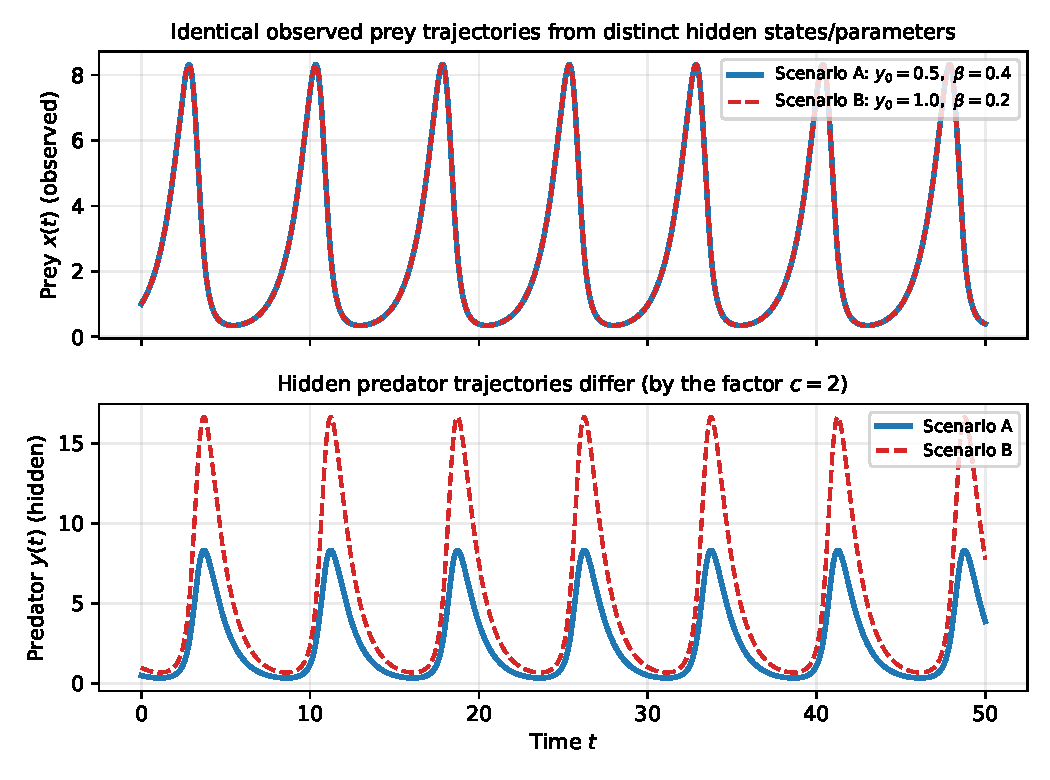
\includegraphics[width=0.82\textwidth]{figures/lv_nonident.pdf}
  %\framebox{\parbox{0.8\textwidth}{\centering
  %  \vspace{3cm}
  %  \textbf{} \\
  %  \small\textit{Identical prey observations $x(t)$ (top) from completely different hidden predator states $y(t)$ and parameter $\beta$ (bottom).}
  %  \vspace{3cm}
  %}}
  \caption{Structural unidentifiability in the Lotka-Volterra model. Scenario A ($x_0=1.0, y_0=0.5, \beta=0.4$) and Scenario B ($x_0=1.0, y_0=1.0, \beta=0.2$) produce identical observable trajectories for the prey $\mathbf{x}_{obs}(t)$ (top), despite originating from completely different hidden predator states and parameters (bottom). This algebraic indistinguishability proves that the full system cannot be identified from partial observations alone.}
  \label{fig:lv_unidentifiable}
\end{figure}

\subsection{OGTT: Jacobian Approximation and Theoretical Observability}
\label{subsec:ident-ogtt}
For the OGTT (oral glucose tolerance test) glucose--insulin minimal model~\cite{ha2025disposition}, the augmented state is
\begin{equation*}
\mathbf{z} = [G, I, N_5, N_6, S_I, \sigma]^\top \in \mathbb{R}^6, \qquad \mathbf{x}_{obs} = \tilde{h}(\mathbf{z}) = G .
\end{equation*}
Due to the high dimensionality and nested recurrences in the vector field, deriving $\mathbf{O}(\mathbf{z})$ even via symbolic computation is intractable.

Instead, we employ a Jacobian-based numerical approximation. The Taylor expansion of the observation $\mathbf{x}_{obs}(t)$ near $t=0$ can be expressed using Lie derivatives:
\begin{equation}
    \mathbf{x}_{obs}(t) = L_{F}^0 \tilde{h}(\mathbf{z}(0)) + t L_{F}^1 \tilde{h}(\mathbf{z}(0)) + \frac{t^2}{2!} L_{F}^2 \tilde{h}(\mathbf{z}(0)) + \dots
\end{equation}
Taking the gradient with respect to the initial augmented state $\mathbf{z}(0)$ and truncating at dimension $d=6$, the Jacobian $\mathbf{J} = \nabla_{\mathbf{z}(0)} \mathbf{x}_{obs}(\mathbf{t})$ evaluated at $T \ge 6$ discrete time points factors into:
\begin{equation}
    \mathbf{J} \approx \underbrace{\begin{bmatrix} 1 & t_1 & \dots & \frac{t_1^{d-1}}{(d-1)!} \\ \vdots & \vdots & \ddots & \vdots \\ 1 & t_T & \dots & \frac{t_T^{d-1}}{(d-1)!} \end{bmatrix}}_{\mathbf{T}} \underbrace{\begin{bmatrix} \nabla_{\mathbf{z}} L_{F}^0 \tilde{h}(\mathbf{z}(0)) \\ \vdots \\ \nabla_{\mathbf{z}} L_{F}^{d-1} \tilde{h}(\mathbf{z}(0)) \end{bmatrix}}_{\mathbf{O}(\mathbf{z}(0))}.
\end{equation}
Since the Vandermonde matrix $\mathbf{T}$ has full column rank for distinct time points, $\text{rank}(\mathbf{J}) = \text{rank}(\mathbf{O}(\mathbf{z}))$. We estimate $\text{rank}(\mathbf{J})$ using finite differences and Singular Value Decomposition (SVD), carefully normalizing the scale of each variable. 

The SVD yields six strictly positive singular values ($\varsigma_1 \approx 1.2\times 10^{2} \dots \varsigma_6 \approx 1.5\times 10^{-3}$; Figure~\ref{fig:ogtt_sensitivity}, left), all well above machine zero (we write $\varsigma$ for singular values to avoid collision with the parameter $\sigma$). This confirms that $\text{rank}(\mathbf{O}) = 6$. Theoretically, under idealized conditions with sufficient time steps and high-order derivative information, the OGTT system is structurally identifiable from glucose alone.

\subsection{Bridging Theory and Practice: The Ill-Conditioning of OGTT}
While theoretically identifiable, the SVD spectrum reveals a critical practical challenge. The singular values span roughly five orders of magnitude, indicating that the Jacobian $\mathbf{J}$ is severely ill-conditioned.

\begin{figure}[htbp]
  \centering
  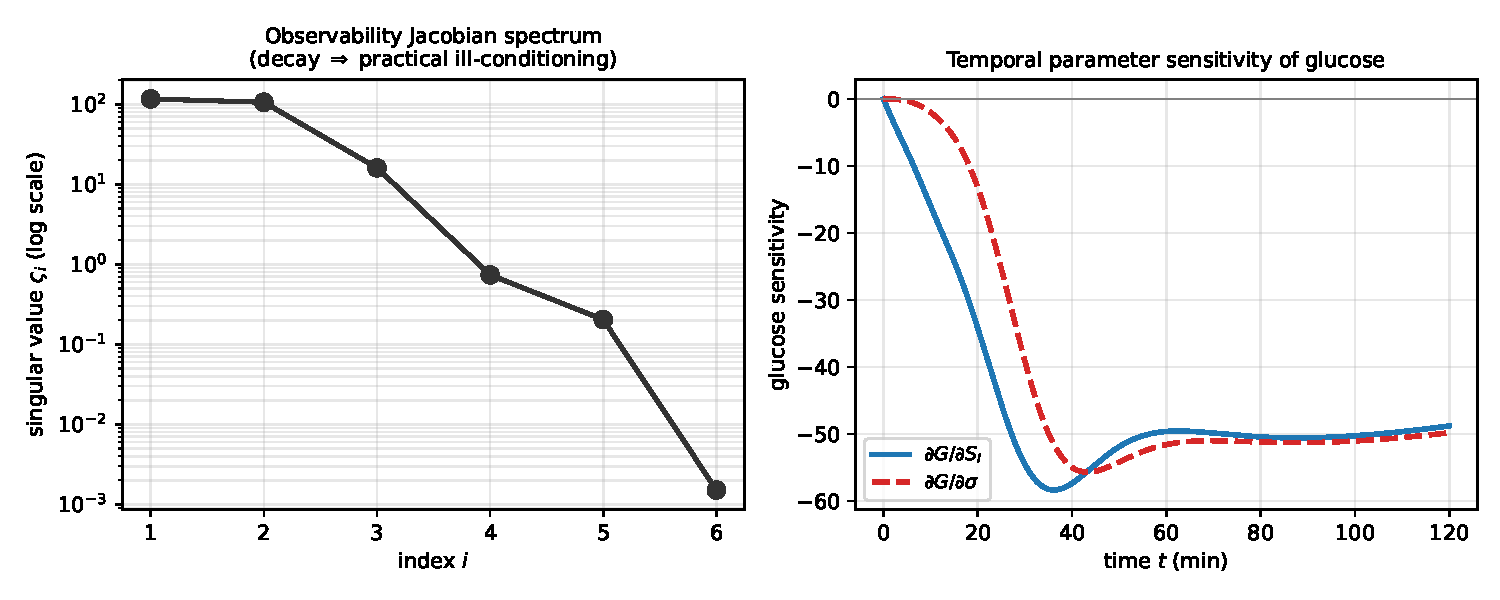
\includegraphics[width=0.92\textwidth]{figures/ogtt_illcond.pdf}
  %\framebox{\parbox{0.8\textwidth}{\centering
  %  \vspace{3cm}
  %  \textbf{} \\
  %  \small\textit{(Left) Singular value spectrum showing steep decay. (Right) Normalized sensitivity dynamics of $S_I$ and $\sigma$ over time.}
  %  \vspace{3cm}
  %}}
  \caption{Ill-conditioning and parameter sensitivity in the OGTT model. (Left) The singular values of the Jacobian decay rapidly, indicating practical unidentifiability despite theoretical full rank. (Right) The temporal sensitivity of glucose to $S_I$ and $\sigma$. Early dynamics ($<30$ min) are dominated by $S_I$, while later dynamics entangle the effects of both parameters.}
  \label{fig:ogtt_sensitivity}
\end{figure}

This ill-conditioning manifests temporally. As shown in Figure \ref{fig:ogtt_sensitivity} (Right), the sensitivity of glucose to insulin sensitivity ($\partial G / \partial S_I$) rises first, becoming strongest within the first $30$--$40$ minutes. The influence of $\beta$-cell function ($\partial G / \partial \sigma$) instead builds up more slowly, along a sigmoid-like profile. In the later stages, the two sensitivities become comparable and the coupled influence of both parameters dictates the glucose trajectory. Under a uniform 30-minute sampling grid without continuous flow information, the neural network struggles to disentangle these intertwined sensitivities. This translates the theoretically full-rank system into a practically unidentifiable regime, severely limiting the precise joint recovery of $(S_I, \sigma)$ and paving the way for the regression-to-mean phenomenon.
